\documentclass{article}
\usepackage{ctex}
\usepackage{tikz}
\begin{document}
    
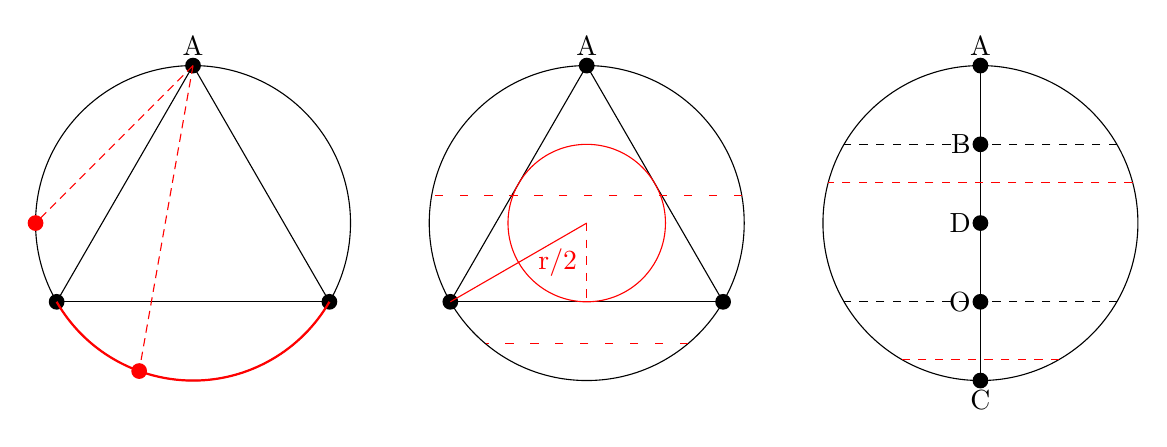
\begin{tikzpicture}

\tikzset{shift={(0,0)}};
\coordinate (a1) at (90:2);
\coordinate (a2) at (210:2);
\coordinate (a3) at (330:2);
\draw (a1)--(a2);
\draw (a1)--(a3);
\draw (a3)--(a2);
\fill (a1) circle (.1) node[above]{A};
\fill (a2) circle (.1);
\fill (a3) circle (.1);
\draw (0,0) circle (2);
\draw[red, thick] (a2) arc (210:330:2);
\fill[red] (250:2) circle (.1); 
\draw[densely dashed,red] (90:2)--(250:2);
\fill[red] (180:2) circle (.1); 
\draw[densely dashed,red] (90:2)--(180:2);


\tikzset{shift={(5,0)}};
\coordinate (b1) at (90:2);
\coordinate (b2) at (210:2);
\coordinate (b3) at (330:2);
\draw (b1)--(b2);
\draw (b1)--(b3);
\draw (b3)--(b2);
\fill (b1) circle (.1) node[above]{A};
\fill (b2) circle (.1);
\fill (b3) circle (.1);
\draw (0,0) circle (2);
\draw[red] (0,0) circle (1);
\draw[red] (0,0)--(b2);
\draw[red, dashed] (0,0)--(-90:1) node[midway,left]{r/2};
\draw[red, loosely dashed] (10:2)--(170:2);
\draw[red, loosely dashed] (-50:2)--(-130:2);

\tikzset{shift={(5,0)}};
\fill (0,2) circle (.1) node[above]{A};
\fill (0,1) circle (.1) node[left]{B};
\fill (0,-1) circle (.1) node[left]{O};
\fill (0,-2) circle (.1) node[below]{C};
\fill (0,0) circle (.1) node[left]{D};
\draw (0,0) circle (2);
\draw[dashed] (30:2)--(150:2);
\draw[dashed] (-30:2)--(-150:2);
\draw (90:2)--(-90:2);
\draw[red, dashed] (15:2)--(165:2);
\draw[red, dashed] (-60:2)--(-120:2);



\end{tikzpicture}

\end{document}